
\def\thoigian{90}%--Thời gian
\de{ĐỀ THI GIỮA HỌC KỲ I NĂM HỌC 2024-2025}{THPT TRẦN PHÚ - Tp Hồ Chí Minh}

\begin{center}
	\textbf{PHẦN 1 - Câu trắc nghiệm nhiều phương án lựa chọn.}
\end{center}
\setcounter{ex}{0}
\Opensolutionfile{ans}[ans-ABCD]
%Câu 1
\begin{ex}%[0H4H2-1][Dự án đề kiểm tra Toán 10 GHKI NH24-25- Hieu Hieu Minh Minh]%[THPT Trần Phú - Tp HCM]
	Cho tam giác $ABC$ biết $b=7$, $c=5$, $\cos A=\dfrac{3}{5}$. Tính cạnh $a$.
	\choice
	{$a=4$}
	{$a=2\sqrt{2}$}
	{\True $a=4\sqrt{2}$}
	{$a=6$}
	\loigiai{
		Ta có $a^2=b^2+c^2-2bc\cos A=7^2+5^2-2\cdot 7 \cdot 5 \cdot \dfrac{3}{5}=32 \Rightarrow c=4\sqrt{2}$.
	}
\end{ex}

%Câu 2
\begin{ex}%[0D3H1-2][Dự án đề kiểm tra Toán 10 GHKI NH24-25- Hieu Hieu Minh Minh]%[THPT Trần Phú - Tp HCM]
	Hàm số nào trong các hàm số dưới đây có tập xác định là $\mathbb{R}$ ?
	\choice
	{$y=\dfrac{2 x-1}{x-2}$}
	{$y=\sqrt{x-1}$}
	{\True $y=\dfrac{\sqrt[3]{x}}{x^2+1}$}
	{$y=\dfrac{x-1}{x^2-2x+1}$}
	\loigiai{
		Vì $\sqrt[3]{x}$ xác định $\forall x \in \mathbb{R}$ và $x^2+1>0, \forall x \in \mathbb{R}$ nên hàm số $y=\dfrac{\sqrt[3]{x}}{x^2+1}$ có tập xác định là $\mathbb{R}$.
	}
\end{ex}

%Câu 3
\begin{ex}%[0D2N1-2][Dự án đề kiểm tra Toán 10 GHKI NH24-25- Hieu Hieu Minh Minh]%[THPT Trần Phú - Tp HCM]
	Cặp số nào sau đây \textbf{không} là nghiệm của bất phương trình $5x-2(y-1) \le 0$?
	\choice
	{$(0;1)$}
	{\True $(1;3)$}
	{$(-1;1)$}
	{$(-1;0)$}
	\loigiai{
		Ta thay $x=1$, $y=3$ vào $5x-2(y-1)=5\cdot 1-2(3-1)=1 > 0$ nên cặp số $(1;3)$ không là nghiệm của bất phương trình $5x-2(y-1) \le 0$.
	}
\end{ex}

%Câu 4
\begin{ex}%[0D1N3-3][Dự án đề kiểm tra Toán 10 GHKI NH24-25- Hieu Hieu Minh Minh]%[THPT Trần Phú - Tp HCM]
	Cho hai tập hợp $A=[-5;3)$, $B=(1;+\infty)$. Khi đó $A \cap B$ là tập nào sau đây?
	\choice
	{\True $(1;3)$}
	{$(1;3]$}
	{$[-5;+\infty)$}
	{$[-5;1]$}
	\loigiai{
		Ta có $A \cap B=(1;3)$.
	}
\end{ex}

%Câu 5
\begin{ex}%[0D2N1-1]%[Dự án đề kiểm tra Toán 10 GHKI NH24-25- Hieu Hieu Minh Minh]%[THPT Trần Phú - Tp HCM]
	Bất phương trình $3x-2(y-x+1)>0$ tương đương với bất phương trình nào sau đây?
	\choice
	{$x-2y-2>0$}
	{$5x-2y-1>0$}
	{\True $5x-2y-2>0$}
	{$4x-2y-2>0$}
	\loigiai{
		Ta có \begin{eqnarray*}
			&&3x-2(y-x+1)>0\\
			&\Leftrightarrow& 3x-2y+2x-2>0\\
			&\Leftrightarrow& 5x-2y-2>0
		\end{eqnarray*}
	}
\end{ex}

%Câu 6
\begin{ex}%[0H4H2-1]%[Dự án đề kiểm tra Toán 10 GHKI NH24-25- Hieu Hieu Minh Minh]%[THPT Trần Phú - Tp HCM]
	Tam giác $ABC$ có $\widehat{A}=120^{\circ}$ thì mệnh đề nào sau đây đúng?
	\choice
	{$a^2=b^2+c^2-3bc$}
	{\True $a^2=b^2+c^2+bc$}
	{$a^2=b^2+c^2+3bc$}
	{$a^2=b^2+c^2+2bc$}
	\loigiai{
		Ta có $a^2=b^2+c^2-2bc\cos A= b^2+c^2-2bc\cdot \cos 120 ^\circ=b^2+c^2+bc$.
	}
\end{ex}

%Câu 7 (Sửa ID và Metadata)
\begin{ex}%[0D1H3-2]%[Dự án đề kiểm tra Toán 10 GHKI NH24-25- Hieu Hieu Minh Minh]%[THPT Trần Phú - Tp HCM]
	Cho tập hợp $A=\left\{x \in \mathbb{Z} \mid 1 \leq x^2 \leq 9\right\}$, tập hợp $B$ là các ước nguyên dương của $6$. Tập hợp $B \setminus A$ bằng tập nào dưới đây?
	\choice
	{$\varnothing$}
	{\True $\{6\}$}
	{$\mathbb{R}$}
	{$\{ \pm 6\}$}
	\loigiai{
		Ta có $A=\left\{x \in \mathbb{Z} \mid 1 \leq x^2 \leq 9\right\}\Rightarrow A=\{\pm 1, \pm 2, \pm 3\}$	và $B=\{1,2,3,6\}$.\\
		Vậy $B\setminus A = \{6\}$.
	}
\end{ex}

%Câu 8
\begin{ex}%[0D3H1-2]%[Dự án đề kiểm tra Toán 10 GHKI NH24-25- Hieu Hieu Minh Minh]%[THPT Trần Phú - Tp HCM]
	Tìm tập xác định $D$ của hàm số $y=\sqrt{3x-9}-3 \sqrt{3+x}$.
	\choice
	{$\mathscr{D}=\mathbb{R} \setminus \left\{\dfrac{1}{3} ; 3\right\}$}
	{$\mathscr{D}=\left[\dfrac{1}{3};3\right]$}
	{$\mathscr{D}=\left(\dfrac{1}{3};3\right)$}
	{\True $\mathscr{D}=[3;+\infty)$}
	\loigiai{
		Điều kiện xác định của hàm số khi và chỉ khi 
		$\heva{&3x-9\ge 0\\&3+x\ge 0}\Leftrightarrow \heva{&x \ge 3\\&x \ge -3}\Leftrightarrow x \ge 3$.\\
		Vậy tập xác định của hàm số đã cho là $\mathscr{D}=[3 ;+\infty)$.
	}
\end{ex}

%Câu 9
\begin{ex}%[0D3N1-3]%[Dự án đề kiểm tra Toán 10 GHKI NH24-25- Hieu Hieu Minh Minh]%[THPT Trần Phú - Tp HCM]
	\immini{Tìm tập giá trị $T$ của hàm số $y=f(x)$ xác định trên đoạn $[-3;2]$ và có đồ thị được biểu diễn bởi hình bên.}{
		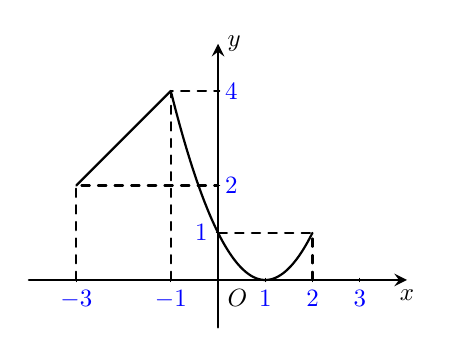
\begin{tikzpicture}[line join = round, line cap = round,>=stealth,thick,scale=0.6]
			\draw[->,line width = 1pt] (-4,0)--(0,0) node[below right]{$O$}--(4,0) node[below]{$x$};
			\draw[->,line width = 1pt] (0,-1)--(0,5) node[right]{$y$};
			\foreach \x in {-3,-1,1,2,3} \draw[thin] (\x,1pt)--(\x,-1pt) node [below,blue] {$\x$};
			\foreach \y in {1} \draw[thin] (1pt,\y)--(-1pt,\y) node [left,blue] {$\y$};
			\foreach \y in {2,4} \draw[thin] (1pt,\y)--(-1pt,\y) node [right,blue] {$\y$};
			\draw[samples=100,domain=-1:2,smooth] plot (\x, {(\x)^2-2*(\x)+1});
			\draw (-3,2)--(-1,4);
			\draw[dashed] (-3,0)--(-3,2)--(0,2) (-1,0)--(-1,4)--(0,4) (2,0)--(2,1)--(0,1);
		\end{tikzpicture}
	}
	\choice
	{$T=[-3;2]$}
	{$\mathrm{T}=(-3;2)$}
	{$T=(0;4)$}
	{\True $T=[0;4]$}
	\loigiai{
		Dựa vào đồ thị hàm số đã cho ta thấy $T=[0;4]$.
	}
\end{ex}

%Câu 10
\begin{ex}%[0D1N2-2]%[Dự án đề kiểm tra Toán 10 GHKI NH24-25- Hieu Hieu Minh Minh]%[THPT Trần Phú - Tp HCM]
	Khẳng định nào sau đây đúng?
	\choice
	{$a \subset\{a;2\}$}
	{$c \notin\{a;b;c\}$}
	{\True $\varnothing \subset\{a;b\}$}
	{$b=\{b\}$}
	\loigiai{
		Ta có $\varnothing \subset\{a;b\}$.
	}
\end{ex}

%Câu 11
\begin{ex}%[0D3N1-5]%[Dự án đề kiểm tra Toán 10 GHKI NH24-25- Hieu Hieu Minh Minh]%[THPT Trần Phú - Tp HCM]
	\immini{Hàm số $y=f(x)$ xác định trên $[-2;4]$ có đồ thị như hình bên dưới.}
	{
		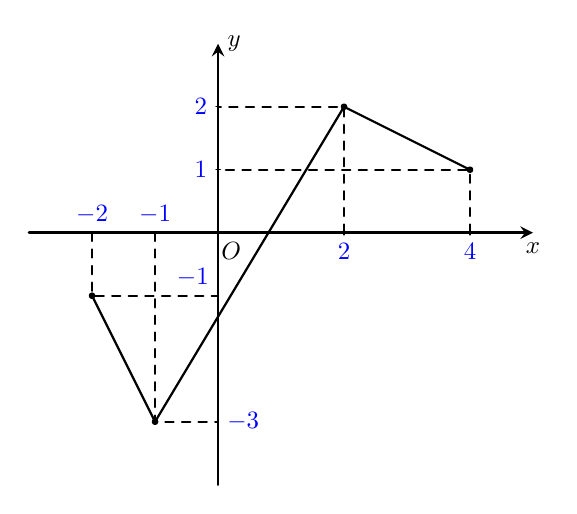
\begin{tikzpicture}[line join = round, line cap = round,>=stealth,thick,scale=0.8]
			\draw[->,line width = 1pt] (-3,0)--(-0.1,0) node[below right]{$O$}--(5,0) node[below]{$x$};
			\draw[->,line width = 1pt] (0,-4)--(0,3) node[right]{$y$};
			\foreach \x in {2,4} \draw[thin] (\x,1pt)--(\x,-1pt) node [below,blue] {$\x$};
			\foreach \y in {1,2} \draw[thin] (1pt,\y)--(-1pt,\y) node [left,blue] {$\y$};
			\node [above,blue] at (-1,0){$-1$};
			\node [above,blue] at (-2,0){$-2$};
			\node [above left,blue] at (0,-1){$-1$};
			\node [right,blue] at (0,-3){$-3$};
			\draw (-2,-1)--(-1,-3)--(2,2)--(4,1);
			\draw[dashed] (-2,0)--(-2,-1)--(0,-1) (-1,0)--(-1,-3)--(0,-3) (2,0)--(2,2)--(0,2) (4,0)--(4,1)--(0,1); 
			\draw[fill=black] (-2,-1)circle(1pt) (-1,-3)circle(1pt) (2,2)circle(1pt) (4,1)circle(1pt); 
		\end{tikzpicture}
	}
	Hàm số nghịch biến trên khoảng nào sau đây
	\choice
	{$(-3;-1)$}
	{$(0;4)$}
	{$(1;2)$}
	{\True $(3;4)$}
	\loigiai{
		Hàm số nghịch biến trên $(3;4) \subset (2;4)$.
	}
\end{ex}

%Câu 12
\begin{ex}%[0H4N2-1]%[Dự án đề kiểm tra Toán 10 GHKI NH24-25- Hieu Hieu Minh Minh]%[THPT Trần Phú - Tp HCM]
	Cho $\triangle ABC$ với các cạnh $AB=c$, $AC=b$, $BC=a$. Gọi $R$, $r$, $S$ lần lượt là bán kính đường tròn ngoại tiếp, nội tiếp và diện tích của tam giác $ABC$. Trong các phát biểu sau, phát biểu nào \textbf{sai}?
	\choice
	{$S=\dfrac{abc}{4 R}$}
	{\True $R=\dfrac{a}{\sin A}$}
	{$S=\dfrac{1}{2} ab \sin C$}
	{$a^2+b^2-c^2=2ab \cos C$}
	\loigiai{
		Theo định lí sin, ta có $\dfrac{a}{\sin A}=2R \Rightarrow R=\dfrac{a}{2\sin A}$.
	}
\end{ex}

\Closesolutionfile{ans}

%\indapan{6}{ans-ABCD}

%\cauds

\begin{center}
	\textbf{PHẦN 2 - Câu trắc nghiệm đúng sai. Trong mỗi ý a,b,c,d ở mỗi câu, thí sinh chọn đúng hoặc sai}
\end{center}
\setcounter{ex}{0}


\Opensolutionfile{ans}[ans-DS]

%%%==============Cau_EX1==============%%%
\begin{ex}%[0H4H2-2]%[Lớp 10 - Ôn tập giữa học kì 1-THPT Trần Phú-TPHCM]%[Phạm Văn Long]
	Cho tam giác $ABC$ biết $a=3$ cm, $b=4$ cm, $\widehat{C}=90^{\circ}$. Các mệnh đề sau đúng hay sai?
	\choiceTF
	{\True $c^2=a^2+b^2-2a b \cos C$}
	{$c=25$ cm}
	{\True $S=6$ cm$^2$}
	{\True $R=\dfrac{c}{2}$ cm}
	\loigiai{
		\begin{itemchoice}
			\itemch \textbf{Đúng}.\\
			Theo định lí Cô-sin ta có $c^2=a^2+b^2-2a b \cos C$.
			\itemch \textbf{Sai}.\\
			Theo định lí Cô-sin ta có 
			\allowdisplaybreaks
			\begin{eqnarray*}
				c^2&=&a^2+b^2-2a b \cos C\\
				&=&3^2+4^2-2\cdot 3 \cdot 4 \cdot \cos 90^\circ\\
				&=&25.
			\end{eqnarray*}
			Vậy $c=5$.
			\itemch \textbf{Đúng}.\\
			Ta có $S_{\triangle ABC}=\dfrac{1}{2}\cdot ab=\dfrac{1}{2}\cdot 3\cdot 4=6$ cm$^2$.
			\itemch \textbf{Đúng}.\\
			Vì $\triangle ABC$ vuông tại $C$ nên $R=\dfrac{c}{2}$.
		\end{itemchoice}
	}
\end{ex}
%%%==============HetCau_EX1==============%%%

%%%==============Cau_EX2==============%%%
\begin{ex}%[0D1V2-3]%[Lớp 10 - Ôn tập giữa học kì 1-THPT Trần Phú-TPHCM]%[Phạm Văn Long]
	Các mệnh đề sau đúng hay sai?
	\choiceTF
	{Số tập con của tập hợp $B=\{2\}$ là $1$}
	{Cho tập hợp $A=\{0; 1; 2; 3; 4\}$, $D=\{x \in \mathbb{R}\mid x-4< 0\}$, Vậy $A\setminus D=\{4\}$}
	{\True Cho tập hợp $A=\{x \in \mathbb{Z} \mid-3\leq x \leq 2\}$, $B=\{x \in \mathbb{R} \mid x+2\leq 0\}$. Ta có tập hợp $A\cap B=\{-3;-2\}$}
	{Cho tập hợp $A=\left\{x \in \mathbb{N} \mid x=6-m^2, m \in \mathbb{N}^*\right\}$. Số phần tử của $A$ bằng $3$}
	\loigiai{
		\begin{itemchoice}
			\itemch \textbf{Sai}.\\
			Tập con của tập hợp $B=\{2\}$ là $\varnothing$ và $B$ nên số tập con là $2$.
			\itemch \textbf{Đúng}.\\
			Ta có $B=(-\infty;4)$.\\
			$A\setminus D=\{4\}$.
			\itemch \textbf{Đúng}.\\
			Ta có $A=\{-3;-2;-1;0;1;2\}$ và $B=(-\infty;-2]$. Khi đó $A\cap B=\{-3;-2\}$.
			\itemch \textbf{Sai}.\\
			Ta có $6-m^2 \in \mathbb{N}$ nên $6-m^2\ge 0 \Rightarrow -\sqrt{6}\le m\le \sqrt{6}$.\\
			Mà $m \in \mathbb{N}^*$ nên $m\in \{1;2\}$.\\
			Suy ra $A=\{5;2\}$. Vậy $A$ có $2$ phần tử.
		\end{itemchoice}
	}
\end{ex}
%%%==============HetCau_EX2==============%%%

%%%==============Cau_EX3==============%%%
\begin{ex}%[0D3H1-5]%[Lớp 10 - Ôn tập giữa học kì 1-THPT Trần Phú-TPHCM]%[Phạm Văn Long]
	Các mệnh đề sau đúng hay sai?
	\choiceTF
	{\True Hàm số $f_1(x)=2x-1$ đồng biến trên khoảng $(2; 5)$}
	{Hàm số $y=f_2(x)=\sqrt{x+3}+\dfrac{\sqrt{-x}}{x+3}$ có tập xác định $\mathscr{D}=(-3; 0)$}
	{Cho hàm số $y=f_3(x)$ nghịch biến trên khoảng $(0;+\infty)$ thì $f(2) < f(3)$}
	{Cho hàm số $y=-3x+5$. Trong bốn điểm $A(-2; 3)$, $B(1; 2)$, $C(0; 5)$, $D(-1; 2)$, không có điểm nào thuộc đồ thị hàm số đã cho}
	\loigiai{
		\begin{itemchoice}
			\itemch \textbf{Đúng}.\\
			Hàm số $f_1(x)=2x-1$ có $a=2>0$ nên đồng biến trên $\mathbb{R}$ do đó đồng biến trên khoảng $(2; 5)$.
			\itemch \textbf{Sai}.\\
			Điều kiện xác định $\heva{&x+3\ge 0\\&-x\ge 0\\&x+3\ne 0}\Leftrightarrow -3<x\le 0$.\\
			Vậy $\mathscr{D}=(-3;0]$.
			\itemch \textbf{Sai}.\\
			Ta có $2<3$ và hàm số $y=f_3(x)$ nghịch biến trên khoảng $(0;+\infty)$ nên $f(2)>f(3)$.
			\itemch \textbf{Sai}.\\
			Ta thấy $B(1; 2)$ thuộc đồ thị hàm số $y=-3x+5$ vì khi $x=1$ thì $y=2$.
		\end{itemchoice}
	}
\end{ex}
%%%==============HetCau_EX3==============%%%

%%%==============Cau_EX4==============%%%
\begin{ex}%[0D2H1-2]%[Lớp 10 - Ôn tập giữa học kì 1-THPT Trần Phú-TPHCM]%[Phạm Văn Long]
	\immini{Biểu diễn miền nghiệm của bất phương trình $$-x+2+2(y-2) < 2(1-x)$$ trên mặt phẳng tọa độ $Oxy$. Ta thực hiện qua các bước sau đúng hay sai?
		\choiceTF
		{\True Biến đổi $-x+2+2(y-2) < 2(1-x) \Leftrightarrow x+2y-4< 0$}
		{\True Vẽ đường thẳng $d\colon x+2y-4=0$ đi qua $A(4; 0)$ và $B(0; 2)$}
		{Ta thấy, gốc $O\notin d$ và $0+2\cdot 0+4=4> 0$}
		{\True Miền nghiệm của bất phương trình là nửa mặt phẳng không kể cả bờ $d$ và chứa gốc tọa độ $O$}}
	{\begin{tikzpicture}[line join=round, line cap=round,>=stealth,thick,scale=0.7]
			\tikzset{every node/.style={scale=0.9}}
			\begin{scope}
				\clip (-2,-1) rectangle (5.0,3.0);
				\fill[pattern=north east lines] (-2,3)--(5,3)--(5,-0.5)--cycle;
				\draw (-2,3)--(5,-0.5) node [pos=0.5,right] {$(d)$};
			\end{scope}
			\draw[->] (-2,0)--(5.0,0) node[above]{$x$};
			\draw[->] (0,-1)--(0,3) node[left]{$y$};
			\draw (0,0) node[below left]{$O$};
			\foreach \x in {1,2,3,4}
			\draw[thin] (\x,1pt)--(\x,-1pt) node [below] {$\x$};
			\foreach \y in {1,2}
			\draw[thin] (1pt,\y)--(-1pt,\y) node [left] {$\y$};
			\draw (0,2.1) node[right]{$B$} (4,0) node[above]{$A$};
	\end{tikzpicture}}
	\loigiai{
		\begin{itemchoice}
			\itemch \textbf{Đúng}.\\
			Ta có $-x+2+2(y-2) < 2(1-x) \Leftrightarrow x+2y-4< 0$.
			\itemch \textbf{Đúng}.\\
			Đường thẳng $d\colon x+2y-4=0$ đi qua $A(4; 0)$ và $B(0; 2)$.
			\itemch \textbf{Sai}.\\
			Ta thấy, gốc $O\in d$ và $0+2\cdot 0-4=-4<0$.
			\itemch \textbf{Đúng}.\\
			Miền nghiệm của bất phương trình là nửa mặt phẳng không kể cả bờ $d$ và chứa gốc tọa độ $O$.
	\end{itemchoice}}
\end{ex}
\Closesolutionfile{ans}



\begin{center}
	\textbf{PHẦN 3 - Phần tự luận}
\end{center}
\setcounter{ex}{0}

\Opensolutionfile{ans}[ans-KQ]

%-----Câu 1
\begin{ex}%[0D1H3-4]%[Lớp 10 - Giữa học kì 1 - THPT Trần Phú]%[Trần Văn Hùng]
	Cho các tập hợp $A=\{x\in \mathbb{N}\mid (2x^2-3x+1)(x^2-4x)=0\}$, $B=\{0;1;2;3\}$, $C=(-3;2)$, $D=(-1;3]$. Tìm $A\cup B$, $B\setminus A$, $C\cap D$, $D\setminus C$.
	\loigiai{
		Ta có $(2x^2-3x+1)(x^2-4x)=0\Leftrightarrow \hoac{&2x^2-3x+1=0\\&x^2-4x=0}\Leftrightarrow \hoac{&x=1\in \mathbb{N}\\&x=\dfrac{1}{2}\not\in \mathbb{N}\\&x=0\in \mathbb{N}\\&x=4\in \mathbb{N}}\Rightarrow A=\{0;1;4\}$.\\
		Suy ra
		\begin{itemize}
			\item $A\cup B=\{0;1;2;3;4\}$.
			\item $B\setminus A=\{2;3\}$.
			\item $C\cap D=(-1;2)$.
			\item $D\setminus C=[2;3]$.
		\end{itemize}
	}
\end{ex}
%-----Câu 2
\begin{ex}%[0H4H3-1]%[Lớp 10 - Giữa học kì 1 - THPT Trần Phú]%[Trần Văn Hùng]
	\immini{
		Gia đình chú Sáu sở hữu một mảnh đất hình tam giác. Chiều dài của hàng rào $MN$ là $150$ m, chiều dài của hàng rào $MP$ là $230$ m. Góc giữa hai hàng rào $MN$ và $MP$ là $120^\circ$.
		\begin{enumEX}{1}
			\item Diện tích mảnh đất mà gia đình chú Sáu sở hữu là bao nhiêu mét vuông?
			\item Chiều dài hàng rào $NP$ là bao nhiêu mét?
		\end{enumEX}
		(\it kết quả làm tròn đến hàng phần trăm)
	}
	{
		\begin{tikzpicture}[scale=1, font=\footnotesize, line join=round, line cap=round, >=stealth]
			\coordinate (P) at (5,1);\coordinate (N) at (0,0);\coordinate (M) at (2,-1); 
			\draw (M)--(N)--(P)--(M);
			\foreach \x/\g in {M/-90,N/180,P/0} \fill[black](\x) circle (1pt) ($(\x)+(\g:4mm)$) node{$\x$};
		\end{tikzpicture}
	}
	
	\loigiai{
		\begin{enumEX}{1}
			\item Diện tích mảnh đất là 
			$$S=\dfrac{1}{2}\cdot MN\cdot MP\sin\widehat{NMP}=\dfrac{1}{2}\cdot 150\cdot 230\cdot\sin 120^\circ=8625\sqrt{3}\approx 14938{,}94\, {\text{m}}^2.$$
			\item Áp dụng định lí côsin trong tam giác $MNP$, suy ra 
			\begin{eqnarray*}
				NP^2&=&MN^2+MP^2-2MN\cdot MP\cos 120^\circ\\
				&=&150^2+230^2-2\cdot 150\cdot 230\cdot \cos120^\circ=109900\\
				\Rightarrow NP&\approx&331{,}51 \, {\text{m}}.
			\end{eqnarray*}
			Vậy chiều dài hàng rào $NP$ là $331{,}51 $ mét.
		\end{enumEX}
	}
\end{ex}
%-----Câu 3
\begin{ex}%[0D2V2-3]%[Lớp 10 - Giữa học kì 1 - THPT Trần Phú]%[Trần Văn Hùng]
	Một nhà máy có hai máy $A$, $B$ sản xuất mì tôm và miến gạo. Một tấn mì tôm lãi $3$ triệu đồng, một tấn miến gạo lãi $2{,}8$ triệu đồng. Muốn sản xuất $1$ tấn mì tôm dùng máy $A$ trong $3$ giờ và máy $B$ trong $1$ giờ. Muốn sản xuất $1$ tấn miến gạo dùng máy $A$ trong $1$ giờ và máy $B$ trong $1$ giờ. Một máy không thể dùng để sản xuất đồng thời cả mì tôm và miến gạo. Máy $A$ làm việc không quá $6$ giờ trong một ngày, máy $B$ một ngày chỉ làm việc không quá $4$ giờ. Hỏi muốn đạt số tiền lãi cao nhất thì  mỗi ngày nhà máy phải sản xuất bao nhiêu tấn mì tôm và bao nhiêu tấn miến gạo?
	\loigiai{
		Gọi $x$, $y$ lần lượt là số tấn mì tôm và miến gạo ($x\ge 0$, $y\ge 0$).\\
		Theo giả thiết suy ra hệ bất phương trình $\heva{&x\ge 0\\&y\ge 0&\\&3x+y\le 6\\&x+y\le 4.} (*)$\\
		\begin{center}
			\begin{tikzpicture}[scale=1.1, font=\footnotesize, line join=round, line cap=round, >=stealth]
				\begin{scope}
					\clip (-1,-1) rectangle (5,5);
					\fill[pattern=north east lines] (0,-1)--(-1,-1)--(-1,5)--(0,5)--cycle;
					\fill[pattern=north east lines] (-1,0)--(-1,-1)--(5,-1)--(5,0)--cycle;
					\fill[pattern=north east lines] (-2,12)--(6,12)--(6,-12)--cycle;
					\fill[pattern=north east lines] (-2,6)--(6,6)--(6,-2)--cycle;
					\draw (0.33,5)--(2.33,-1) node [pos=0.65, above, sloped] {$3x+y-6=0$};
					\draw (-1,5)--(5,-1) node [pos=0.45, above, sloped] {$x+y-4=0$};
					\draw[fill] (0,4) circle(1pt)  (1,3) node [left] {$B$} circle(1pt) (2,0) node [above left] {$C$} circle(1pt);
					\draw (0.1,3.9) node [below] {$A$};
				\end{scope}
				\draw[->] (-1,0)--(5,0) node[below]{$x$};
				\draw[->] (0,-1)--(0,5) node[left]{$y$};
				\draw (0,0) node[below left]{$O$};
				\foreach \x in {1,2,4}
				\draw[thin] (\x,1pt)--(\x,-1pt) node [below] {$\x$};
				\foreach \y in {3,4}
				\draw[thin] (1pt,\y)--(-1pt,\y) node [left] {$\y$};
			\end{tikzpicture}
		\end{center}
		Biểu diễn miền nghiệm của hệ $(*)$ ta được miền nghiệm của hệ $(*)$ là tứ giác $OABC$ trong đó $O(0;0)$, $A(0;4)$, $B(1;3)$, $C(2;0)$.\\
		Số tiền lãi mỗi ngày là $T(x;y)=3x+2{,}8y$ (triệu đồng).\\
		Thay tọa độ điểm $O$, $A$, $B$, $C$ vào biểu thức $T$.\\
		Ta có $T(0;0)=0$, $T(0;4)=11{,}2$, $T(1;3)=11{,}4$, $T(2;0)=6$.\\
		Vậy số tiền lãi cao nhất là $T=11{,}4$ triệu đồng khi mỗi ngày sản xuất $1$ tấn mì tôm và $3$ tấn miến gạo.
	}
\end{ex}

\Closesolutionfile{ans}

